\documentclass{article}
\usepackage{tikz}
\usetikzlibrary{arrows.meta,positioning,calc,shapes.geometric}
\pagestyle{empty}
\begin{document}
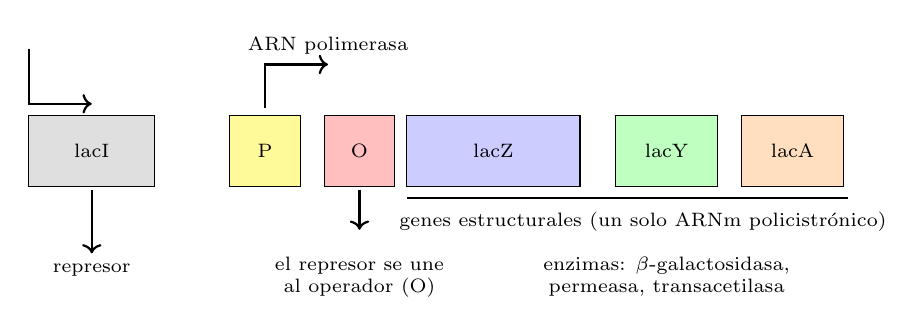
\begin{tikzpicture}
\tikzset{every node/.append style={align=center}}

\def\gene#1#2#3#4{\node[draw, fill=#4, minimum width=#2cm, minimum height=0.9cm, font=\scriptsize] at (#1,0) {#3};}
\gene{0.0}{1.6}{lacI}{gray!25}\gene{2.2}{0.9}{P}{yellow!40}\gene{3.4}{0.9}{O}{red!25}
\gene{5.1}{2.2}{lacZ}{blue!20}\gene{7.3}{1.3}{lacY}{green!25}\gene{8.9}{1.3}{lacA}{orange!25}
\draw[->, thick] (-0.8,1.3) -- (-0.8,0.6) -- (0.0,0.6); 
\draw[->, thick] (0.0,-0.5) -- (0.0,-1.3) node[below, font=\scriptsize] {represor};
\draw[->, thick] (3.4,-0.5) -- (3.4,-1.0); \node[font=\scriptsize, align=center] at (3.4,-1.6) {el represor se une\\ al operador (O)};
\draw[thick, ->] (2.2,0.55) -- (2.2,1.1) -- (3.0,1.1) node[above, font=\scriptsize] {ARN polimerasa};
\node[font=\scriptsize, align=center] at (7.3,-1.6) {enzimas: $\beta$-galactosidasa,\\ permeasa, transacetilasa};
\draw[thick] (4.0,-0.6) -- (9.6,-0.6);
\node[font=\scriptsize] at (7.0,-0.9) {genes estructurales (un solo ARNm policistrónico)};

\end{tikzpicture}
\end{document}
